\chapter{初段ミューオントリガーシステム}
本章では、ATLAS トリガーシステムの一つである初段ミューオントリガーシステムに着目し、Run-3 におけるエンドキャプ部初段ミューオントリガーシステムについて述べる。

\section{ATLAS トリガーシステムの概要}
ATLAS 実験では、LHC を用いて 40 MHz での陽子陽子衝突の測定を行っている。しかし、データ記憶容量の制限が存在するためすべての衝突事象を保存することはできず、現在の制約ではトリガーレートを約 1 kHz まで削減する必要がある。
そのため、膨大なデータの中から物理として興味のある事象のみを効率よく取得するトリガーシステムを用いて事象選別を行っている。

ATLAS 検出器では、ハードウェアにより高速にトリガー判定を行う初段の Level-1 Trigger (L1 Trigger)、ソフトウェアで詳細なトリガー判定を行う後段の High-Level Trigger (HLT) で構成される2段階のトリガーシステムを用いている。

\subsubsection{Level-1 Trigger}
初段トリガーである Level-1 Trigger では、ATLAS 検出器から送られてくる 40 MHz イベントレートの事象を 2.5 $\mu s$ 以内にトリガー判定を行い、100 kHz まで落とす必要がある。L1 Trigger は高速でのデータ処理を行うために Application Specific Integrated Circuit (ASIC)や Field Programmable Gate Array (FPGA) で構成されるハードウェアに実装されている。
ASIC と FPGA は共に半導体集積回路 (IC) の一種であり、高速・低消費電力で特定の処理を行うように設計が可能である。
ASIC は特定の用途向けに複数の回路を1つにまとめたもので、高速な動作速度や低い消費電力を実現できる。FPGA は ASIC と同様に特定の処理を行うように設計可能で何度でも書き換え可能な集積回路である。

\begin{figure}[tb]
  \centering
  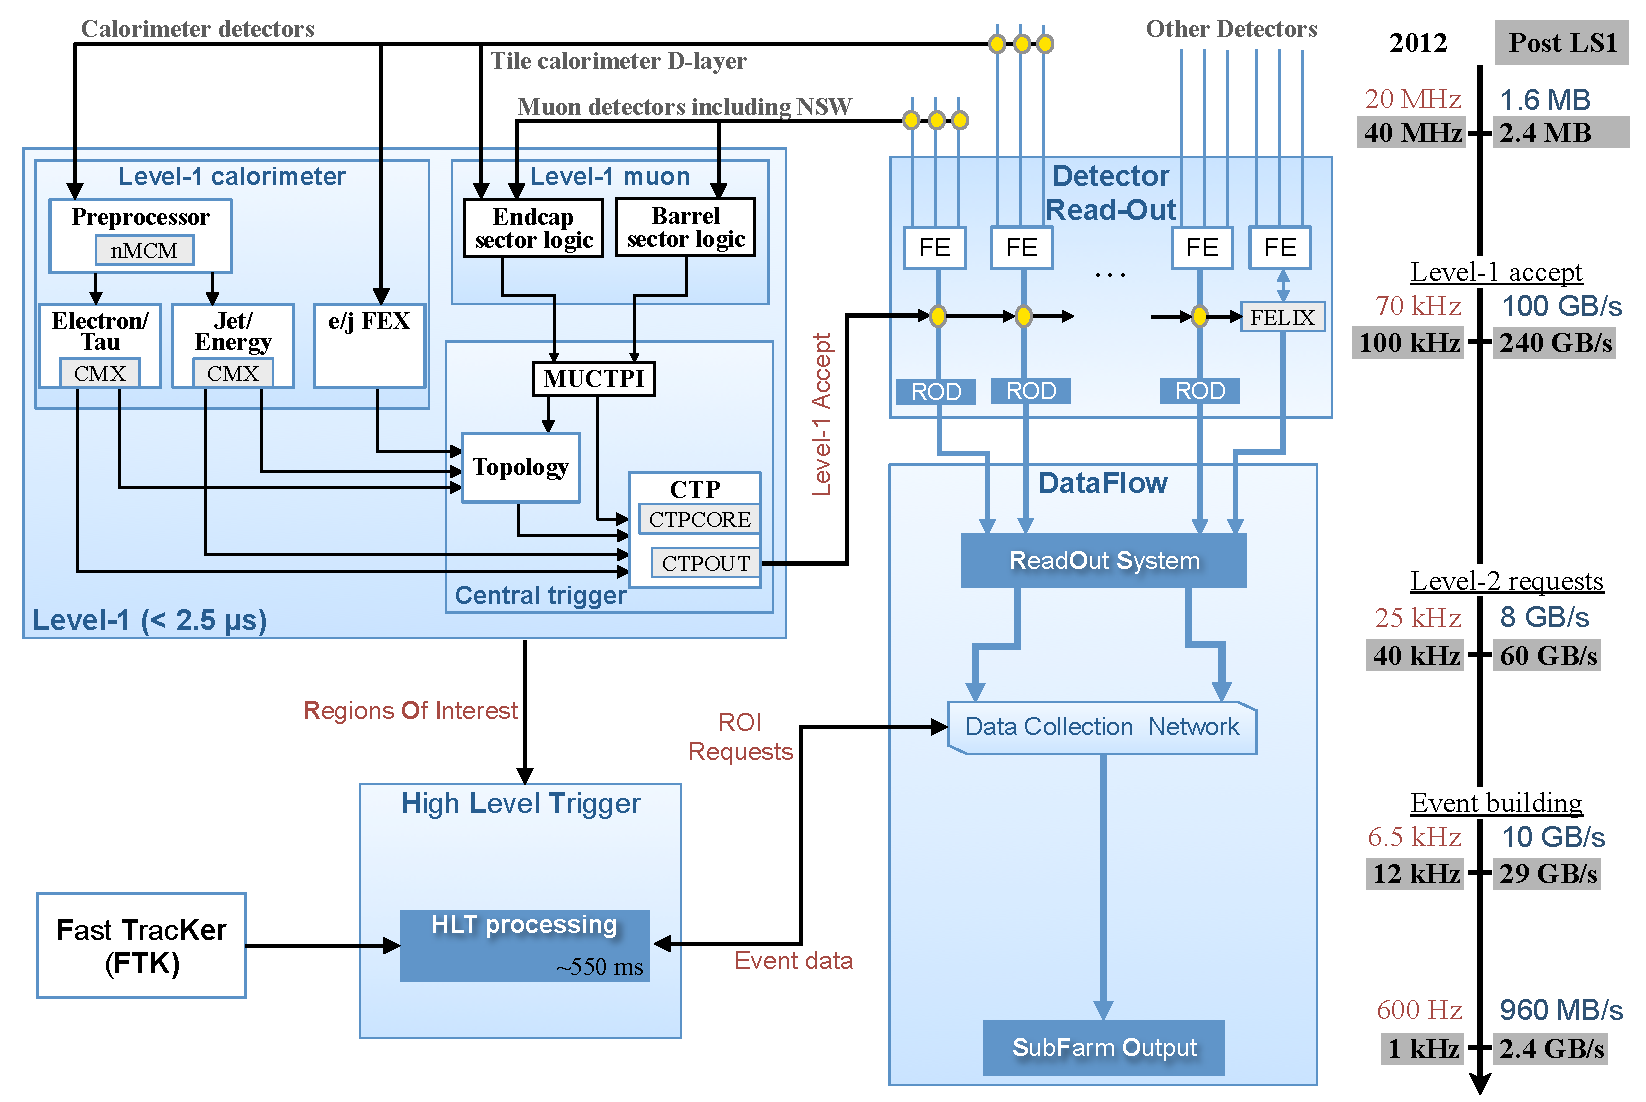
\includegraphics[clip, width=14cm]{fig/3/trigger-nagare2.pdf}
  \caption{Run-3 における ATLAS トリガーシステムの全体像。L1 には L1Calo、L1Muon、L1Topo の 3種類が存在する}
  \label{fig:トリガーの全体像}
\end{figure}

図\ref{fig:トリガーの全体像}に示すように、L1 はカロリメータの情報を用いてトリガー判定を行う L1Calo、ミューオン検出器の情報を用いてトリガー判定を行う L1Muon に加え、これらを組み合わせた複合的なトリガーである Central Trigger から構成されている。L1 では、初めにカロリメータとミューオン検出器の情報からそれぞれ単独にトリガー判定を行う。

L1Calo は電磁カロリメータとハドロンカロリメータの情報を統合してトリガー判定を行う。
カロリメータからの信号は electron FEX (eFEX)、jet FEX (jFEX) 及び global FEX (gFEX) へと送られる。送られた信号はそれぞれ処理が行われ、電子/光子と τ 候補、ジェット候補の判定を行う。

L1Muon はバレル部の RPC とエンドキャップ部の TGC から情報を受け取り、それぞれ独立にトリガー判定を行う。バレル部とエンドキャップ部で独立に判定された L1Muon の情報はMuon-to-CTP interface (MUCTPI) で統合される。

その後、L1Calo と L1Muon からの情報は Central Trigger Processor (CTP) に送られるのと同時に、TopologyProcessor (L1Topo) に送られる。L1Topo では L1Muon と L1Calo の情報を組み合わせて、それぞれの情報から複合的なトリガーを発行する。
最後に L1Muon、L1Calo、L1Topo の情報は CTP に集められ、100 kHz に収まるようにプリスケールをかけられた後に L1Accept (L1A)としてトリガー発行される。

L1 Trigger では、衝突事象が起きてからトリガーの判定を行うまでの間、フロントエンド回路上の buffer で常に一定の時間データを保持している。
L1A 信号を受け取った場合にはデータを後段の ReadOut Driver (ROD) に送られる仕組みとなっている。

L1 Trigger は発行されたトリガーの位置情報 (η, φ) を含む Region of Interest (RoI) を後段の HLT に出力する。HLT では送られてきた RoI の情報から検出器情報を読み出し、より精密なトリガーの判定を行う。

\subsubsection{High-Level Trigger}
High-Level Trigger (HLT) は、L1 Trigger で出力された RoI の情報を用いて、ソフトウェアを用いたオフライン解析に近いアルゴリズムで粒子の再構成することにより、Level-1 Trigger より精密なトリガー判定を行う。
HLT では、L1 Trigger で用いられなかった内部飛跡検出器の情報、MDT や CSC などの精密測定用のミューオン検出器の情報、L1Calo のカロリメータの情報などを用いて、飛跡再構成やより高精度な $E_T$、$p_T$ の計算を行う。トリガーレートは HLT を用いて最終的に数 kHz まで削減される。




\section{Run-3におけるエンドキャプ部初段ミューオントリガー}
ATLAS 検出器でのミューオントリガーは、図\ref{fig:muon}に示すように RPC を用いるバレル部と TGC を用いるエンドキャップ部に分かれている。以下では TGC を用いるエンドキャップ部でのトリガーシステムについて説明する。エンドキャプ部はさらに2つの領域に分けられ、$1.05 < |\eta| < 1.9$ をエンドキャップ領域、$1.9 < |\eta| < 2.4$ をフォワード領域と呼ぶ。

\begin{figure}[tb]
  \centering
  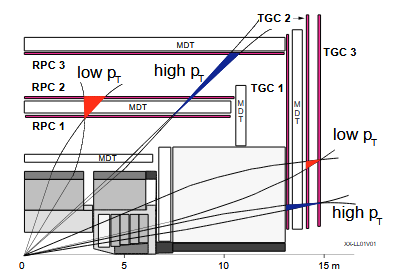
\includegraphics[clip, width=14cm]{fig/3/muon_trigger_overview.png}
  \caption{初段ミューオントリガーに用いる検出器の設置位置。}
  \label{fig:muon}
\end{figure}

\subsection{トリガーセクター}
TGC のトリガー判定に用いられる単位の模式図を図\ref{fig:RoI}に示す。TGC のトリガー判定はトリガーセクターごとに行われ、領域内のミューオンの情報から判定結果が出される。
エンドキャップ部のトリガーセクターは、 $\phi$ 方向にエンドキャプ領域では 48 個、フォワード領域では 24 個に分割している。
これらのトリガーセクターはさらに小さな領域である Region of Interest (RoI) に分割される。RoI は TGC の持つミューオンの位置情報の単位である。
図\ref{fig:RoI} に示すように、エンドキャップ領域のトリガーセクターは $\eta$ 方向に 37 分割、$\phi$ 方向に 4 分割されるため 148 個の RoI で構成されている。フォワード領域のトリガーセクターは $\eta$ 方向に 16 分割、$\phi$ 方向に 4 分割されるため 64 個の RoI で構成されている。また RoI を $\eta$ 方向に 2 つ、$\phi$ 方向に 4 つまとめたものを Sub Sector Cluster (SSC) と呼ぶ。

\begin{figure}[tb]
  \centering
  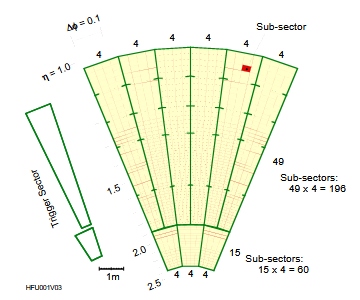
\includegraphics[clip, width=10cm]{fig/3/RoI.png}
  \caption{RoI}
  \label{fig:RoI}
\end{figure}


\subsection{ミューオンの運動量の算出}
エンドキャップ部初段ミューオントリガーで用いられるトリガー判定の概要を図\ref{fig:trigger-scheme}に示す。
衝突点で生成されたミューオンはトロイド磁石の磁場領域より内側にある検出器を通過した後、トロイド磁場領域を通り TGC に到達する。トロイド磁石による磁場は $\phi$ 方向にかかっているため、ミューオンの飛跡はトロイド磁場中で$\eta$ 方向に曲げられる。さらに、衝突点付近のソレノイド磁石で生じる $z$ 方向の磁場成分と、トロイド磁石付近で生じた $R$ 方向の磁場成分によって、ミューオンの飛跡は $\phi$ 方向にも曲げられる。ミューオンの飛跡の曲がり具合は 横方向運動量$p_T$ の大きさによって変化するため、飛跡情報からミューオンの$p_T$を算出することができ、トリガー判定に使用することができる。

トロイド磁場によって曲げられたミューオンは TGC BW のM1, M2, M3 にヒットを残す。ここで、衝突点と M3 のヒット位置を結んだ直線をミューオンが無限運動量で通過したと仮定した場合の飛跡として扱う。この無限運動量を持つミューオンの飛跡と磁場によって曲げられた実際の飛跡を比較し、M1 におけるヒット位置の $R$ 方向と $\phi$ 方向のずれ $dR$、$d\phi$ を計算する。
そして、あらかじめ準備した $dR$、$d\phi$ と $p_T$ の Look-Up Table (LUT) を参照する事で $p_T$ を出力する。

\begin{figure}[tb]
  \centering
  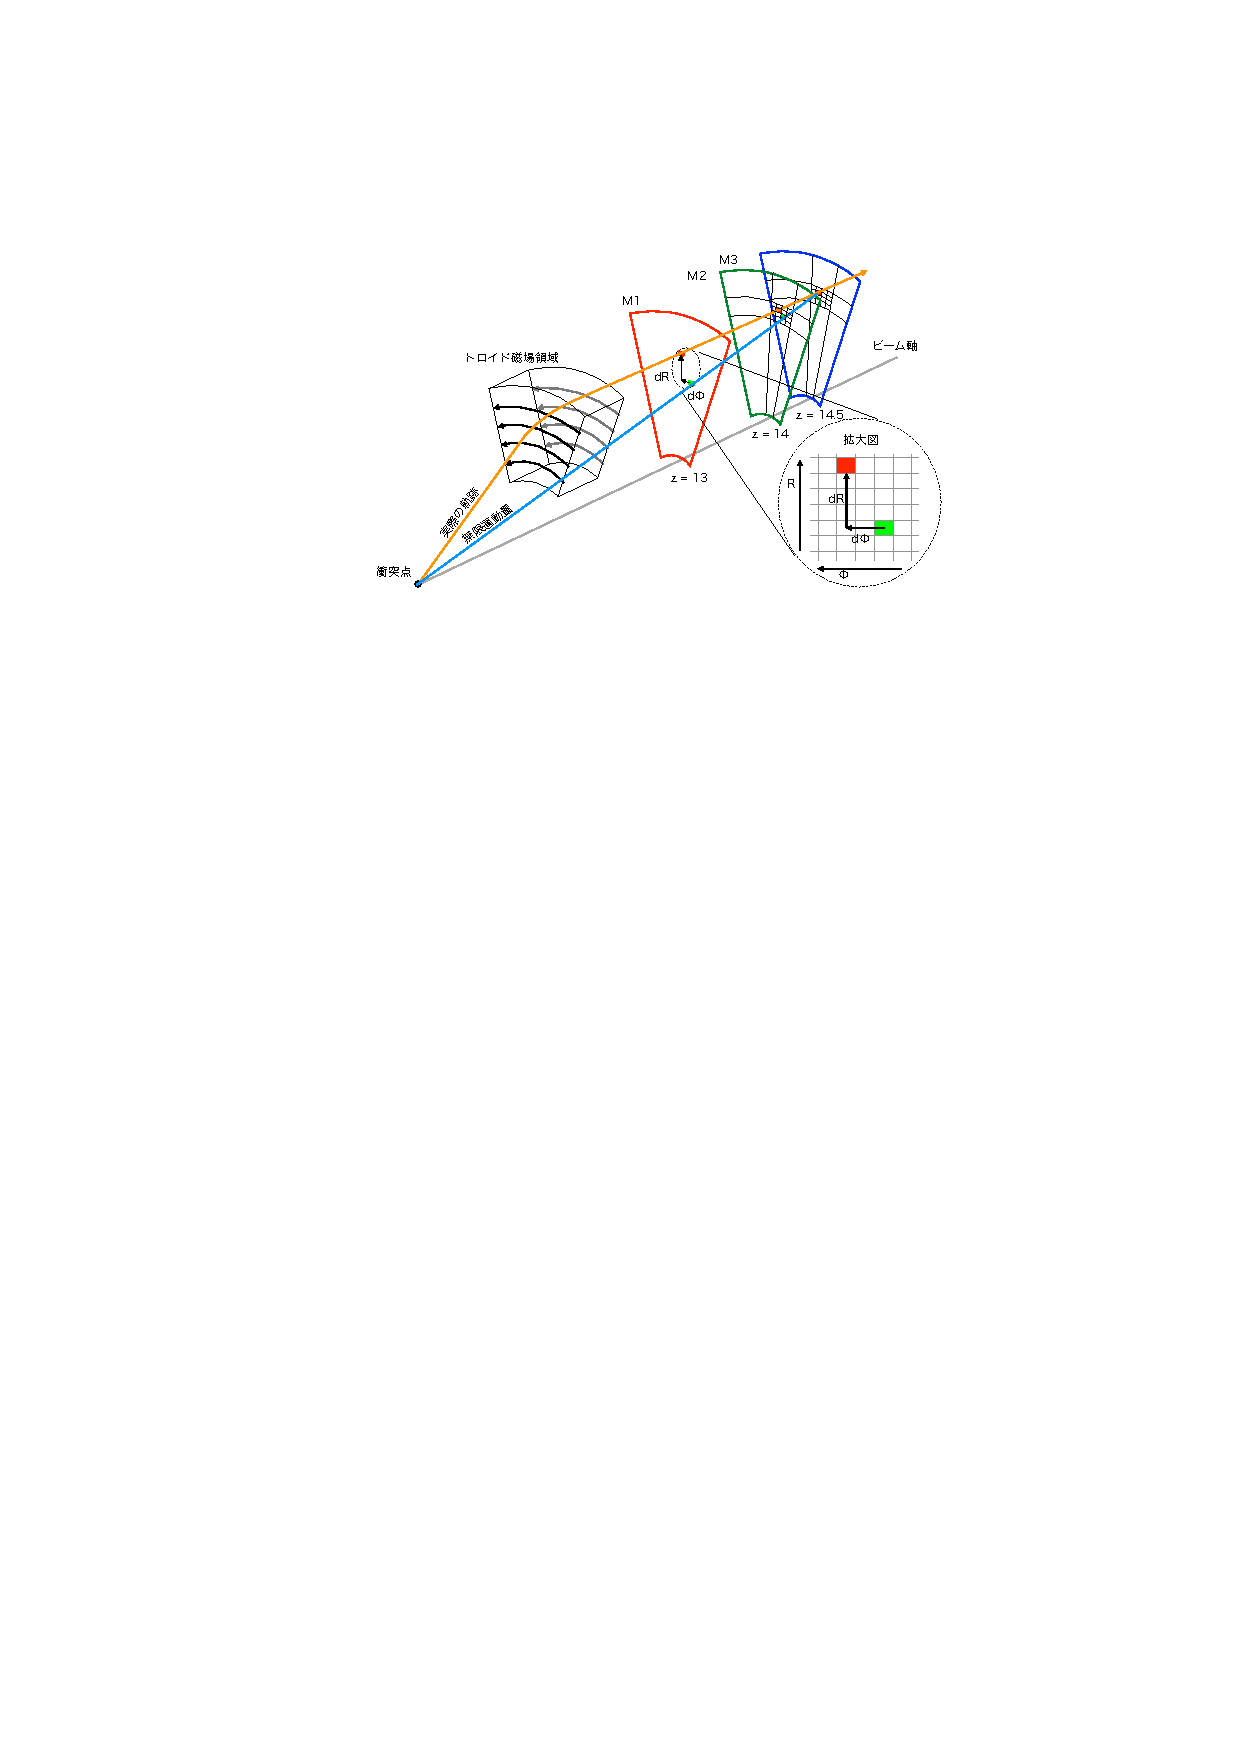
\includegraphics[clip, width=15cm]{fig/3/akatsuka_mt_trigger_scheme.pdf}
  \caption{ATLAS検出器エンドキャップ領域におけるトリガースキームの概念図\cite{article:akatsuka-mron}。無限大の運動量を持つミューオンを仮定し、磁場によって曲げられたミューオンとの位置の差を用いて$p_T$を計算する。}
  \label{fig:trigger-scheme}
\end{figure}

\subsection{Coincidence Window (CW)}\label{section:CW}
$dR$、$d\phi$ と $p_T$ の参照表は Coincidence Window (CW) と呼ばれており、
あらかじめ MC サンプルや実際の測定データを用いて$dR$、$d\phi$に対応する $p_T$ を算出し、図\ref{fig:CW}のような形で保存されている LUT である。
実際の運用では CW は FPGA に LUT 上に実装されており、L1 Trigger でのトリガー判定の際に参照することで高速なトリガー判定を可能にしている。
エンドキャップ部のトロイド磁場や TGC は理想的には 8 回対称だが、磁場の向きや TGC チェンバーの設置位置のずれなどがあるため、CW は TGC BW のすべての単位位置情報 (RoI) ごとに作成されている。
Run-3で使用される CW は図\ref{fig:CW}のように 15 個に分類されており、これが15 段階の $p_T$ 閾値に対応しており、各 $p_T$ 閾値に付された符号はミューオンの電荷に対応している。図のマスの中の数字は表\ref{pt_number} に示す pt number と対応している。



\begin{figure}[tb]
  \centering
  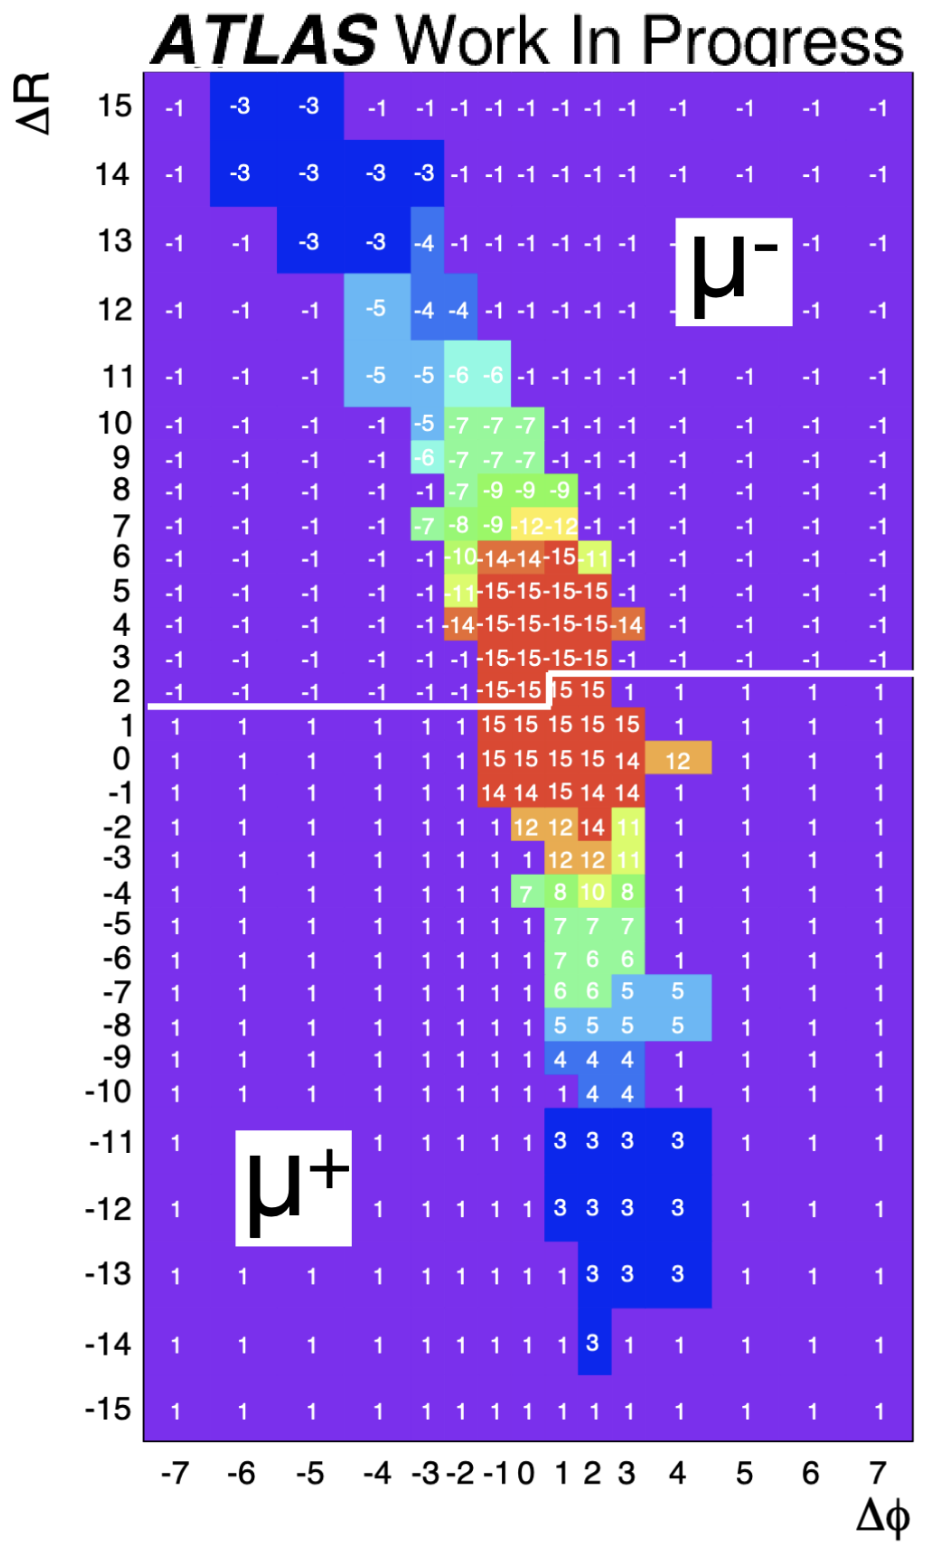
\includegraphics[clip, width=7cm]{fig/3/cw_run3_shiomi.png}
  \caption{Run-3 での TGC における Coincidence Window の例。ミューオンのヒットがあった時にそれぞれの RoI の CW を参照し、$dR$、$dφ$ から $p_T$ を見積もる。}
  \label{fig:CW}
\end{figure}

\begin{table}[tb]
    \caption{Run-3 における 15 段階の $p_T$ の値。}
    \label{pt_number}
    \centering
    \begin{tabular}{|c|c|c|c|c|c|c|c|c|c|c|c|c|c|c|c|c|c|c|c|c|c|c|c|}
        \hline
        $p_t$ number & 1 & 2 & 3 & 4 & 5 & 6 & 7 & 8 & 9 & 10 & 11 & 12 & 13 & 14 & 15\\
        \hline
        $p_T$ [GeV] & 3 & 4 & 5 & 6 & 7 & 8 & 9 & 10 & 11 & 12 & 13 & 14 & 15 & 18 & 20\\
        \hline
    \end{tabular}
\end{table}



\section{2022年 Run-3 における初段ミューオントリガーの性能}
本節では2022年 Run-3 で使用されている CW のトリガー性能について述べる。

\subsection{解析手法}
実際の実験データはトリガーによって選別された粒子の情報のみが保存されているため、そのままのデータを用いてトリガーの性能評価や解析を行うとバイアスがかかる可能性がある。そこで解析の手法として Tag$\&$Probe 法を用いる。

本研究では、内部飛跡検出器とミューオン検出器でそれぞれ独立に再構成され、その後飛跡が結合できたZ ボソン由来のミューオン候補を用いて評価を行う。1回の衝突事象に対し、2 つ以上のミューオン候補が存在するイベントのみを用いる。それらのミューオン候補のうち、任意の2つの電荷が異符号となっているミューオンペアを選び出し、不変質量を再構成する。再構成の条件は、$80 GeV < M_Z < 100 GeV$ とする。
これらのミューオンのうち、一方を Tag ミューオン、もう一方を Probe ミューオンと定義する。
まず、Tag ミューオンがトリガーを発行したかどうかを判定する。Run-2 での実験データを解析に使用する際のトリガー判定には、HLT のシングルミューオントリガーである 「HLT$\_$mu26$\_$ivarmeduium」 を使用する。
ここでトリガー発行の判定を行うために $\Delta R = \sqrt{(\Delta \eta)2 + (\Delta \phi)2}$ を定義する。ここで $\Delta \eta$, $\Delta \phi$ はそれぞれデータの保存されているトリガーを発行した飛跡と Tag ミューオンの $\eta$ 方向、$\phi$ 方向の差である。図\ref{fig:tag_HLT}にTag ミューオンと HLT の $\Delta R$ 分布を示す。本研究では$\Delta R < 0.001$ を満たせば Tag ミューオンがトリガーを発行したとみなす。Tag ミューオンが HLT を発行しているとみなされた時、もう一つのミューオンを Probe ミューオンとして解析に使用する。

\begin{figure}[tb]
  \centering
  \rule{8cm}{6cm}
  \caption{Tag ミューオンと HLT の $\Delta R$ 分布。$\Delta R < 0.005$ ならば Tag ミューオンが HLT を発行したものとする。}
  \label{fig:tag_HLT}
\end{figure}

Probe ミューオンは正しく再構成され、発行されたトリガーとは独立なミューオンである。
Probe ミューオンを使用してエンドキャプ部のトリガー性能を評価するために、Probe ミューオンと TGC のヒット情報を一致させる。図\ref{fig:Probe_TGC}に Probe ミューオンと TGC のヒット情報 の $\Delta R$ 分布を示す。本研究では$\Delta R < 0.04$ を満たせば Probe ミューオンが TGC のヒット情報と一致したものとする。
Probe ミューオンの情報とこのミューオンと一致したTGC のヒット情報を使って解析を行う。

\begin{figure}[tb]
  \centering
  \rule{8cm}{6cm}
  \caption{Probe ミューオンと TGC のヒット情報との $\Delta R$ 分布。$\Delta R < 0.005$ ならば Probe ミューオンが TGC のヒット情報と一致したものとする。}
  \label{fig:Probe_TGC}
\end{figure}


\subsection{トリガーの効率の算出}
トリガー効率$\epsilon$について式\ref{equ:Eff}を用いて評価を行う。
ここで、全ミューオン数はTGC にヒットした全オフラインミューオンと定義し、その中でトリガーを発行したミューオンの数を調べ、トリガー効率を計算する。
\begin{equation}
 \epsilon=\frac{トリガーを発行したミューオンの数}{全ミューオンの数}
 \label{equ:Eff}
\end{equation}

シングルミューオンのシミュレーションサンプルに対してトリガー効率を計算し、2022年Run-3 で使用されているトリガーの各閾値におけるトリガー効率を pT の関数として表した結果を図\ref{fig:Run3_15_MC}に示す。

\begin{figure}[tb]
  \centering
  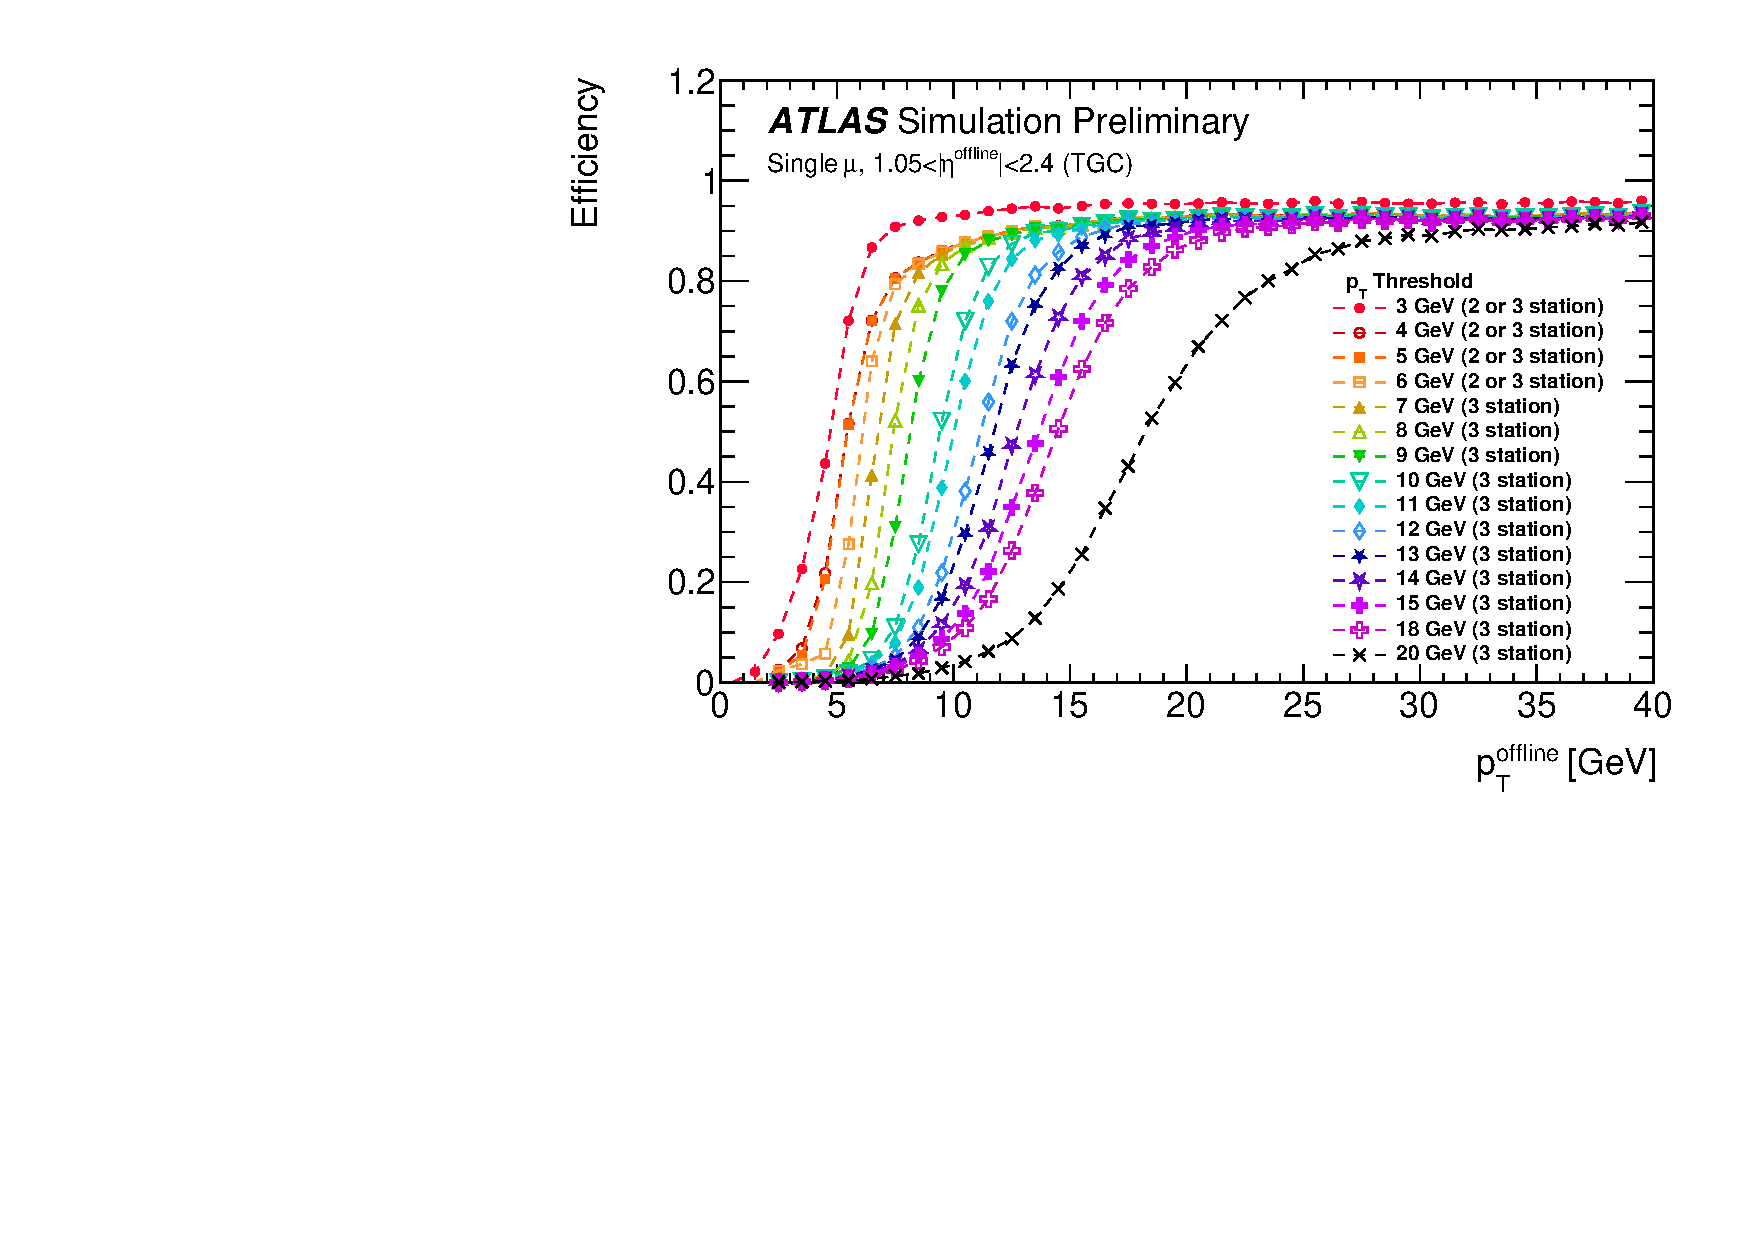
\includegraphics[clip, width=15cm]{fig/3/PLOT-TRIG-2020-01-fig1.pdf}
  \caption{Run-3 における15段階閾値のTurn-on curve。シングルミューオンのシミュレーションサンプルに対してのトリガー効率を示している。}
  \label{fig:Run3_15_MC}
\end{figure}

また、Run-3 の実データに対してトリガー効率を計算し、各閾値におけるトリガー効率を pT の関数として表した結果を図\ref{fig:Run3_15_Data}に示す。

\begin{figure}[tb]
  \centering
  \rule{8cm}{6cm}
  \caption{Run-3 における15段階閾値のTurn-on curve。Run-3 の実データに対してのトリガー効率を示している。}
  \label{fig:Run3_15_Data}
\end{figure}

さらに、各チェンバーごとの各閾値におけるトリガー効率を図\ref{fig:Run3_15_Data_chamber1}に示す。

\begin{figure}
    \centering
    \begin{minipage}[b]{0.4\linewidth}
        \centering
        %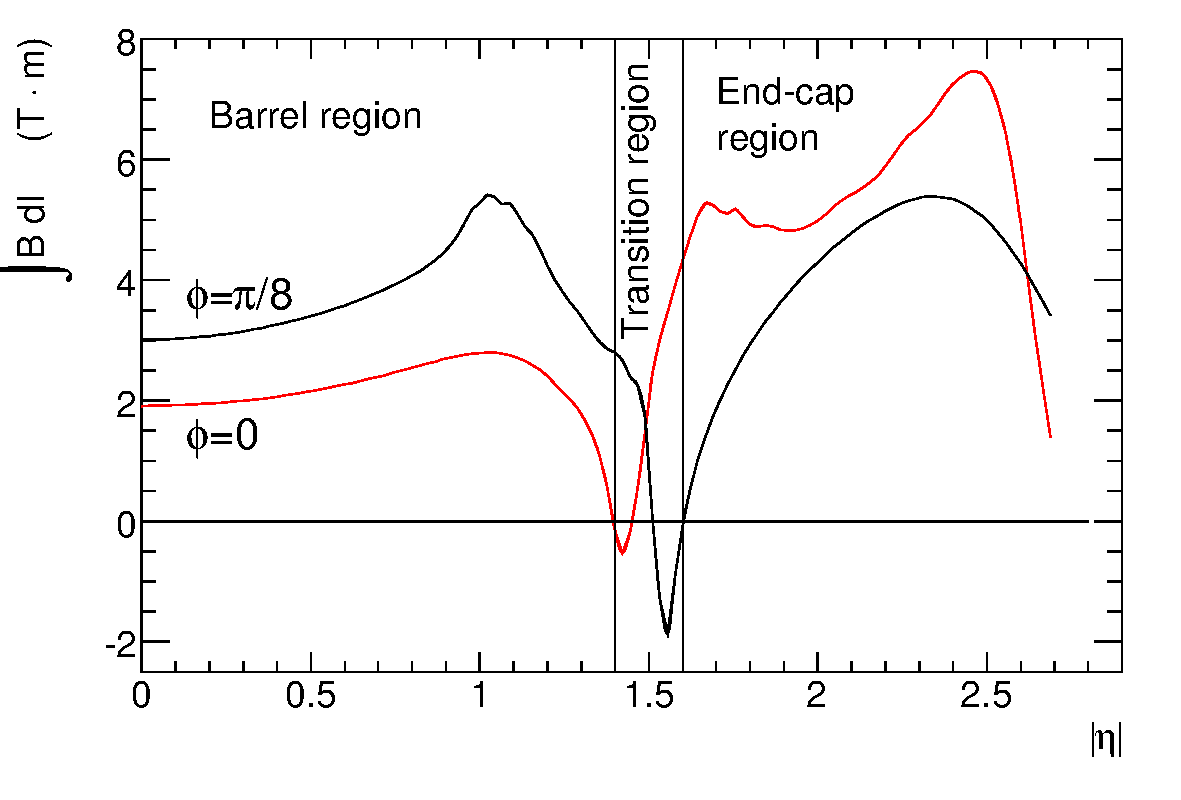
\includegraphics[clip, width=7cm]{fig/2/IBdl.pdf}
        \rule{6cm}{4cm}
        \vspace{10pt}
        \subcaption{}
        \label{}
    \end{minipage}
    \hfill
    \begin{minipage}[b]{0.4\linewidth}
        \centering
        %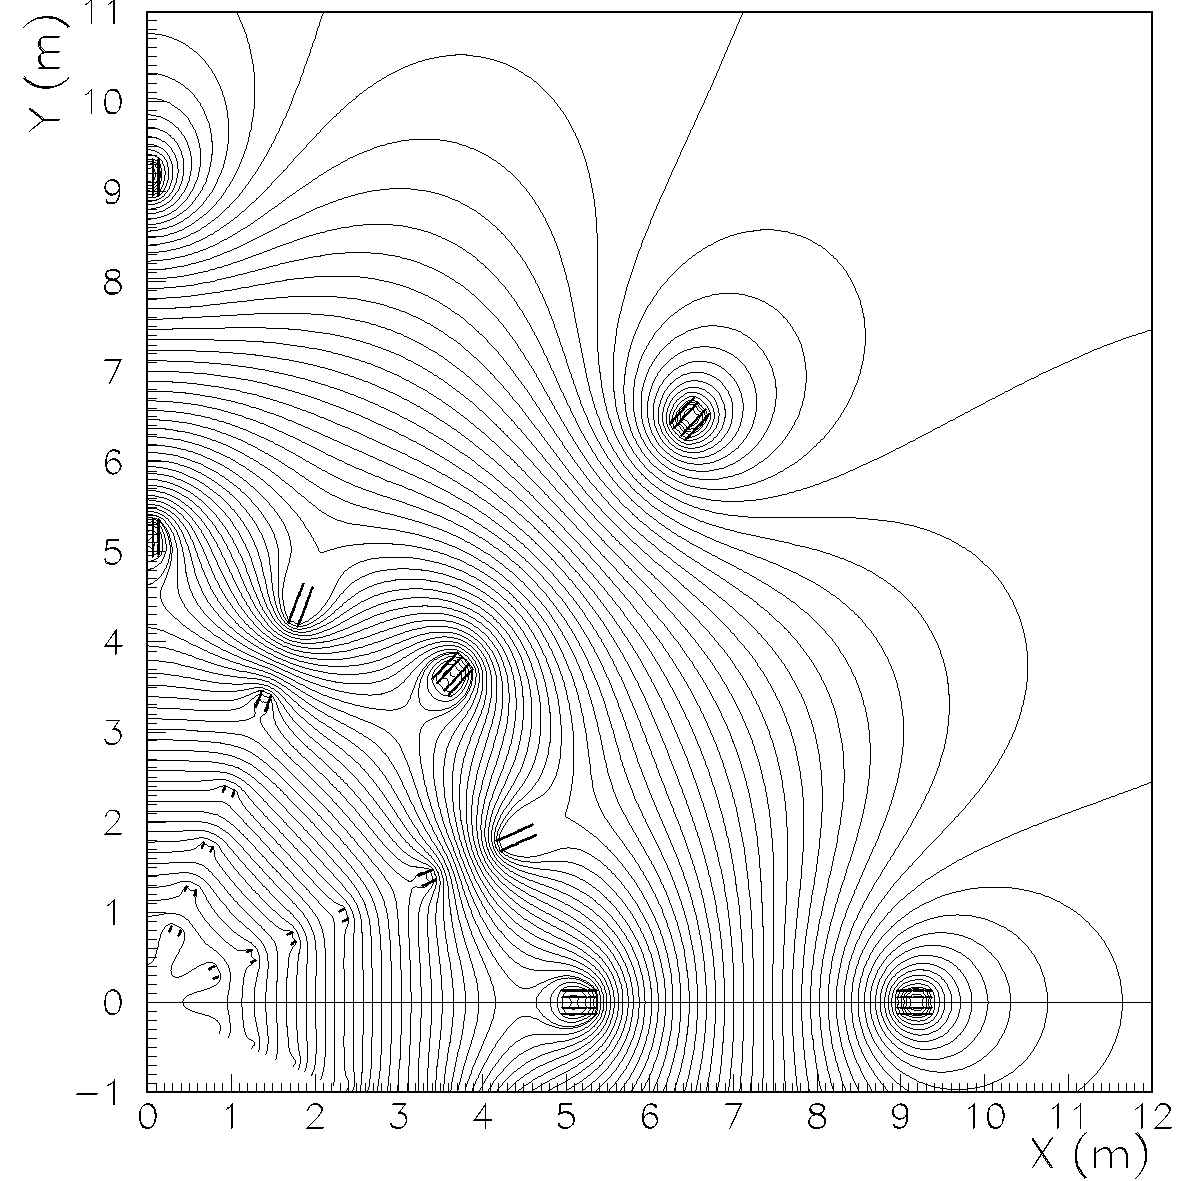
\includegraphics[clip, width=6cm]{fig/2/FMBmap.pdf}
        \rule{6cm}{4cm}
        \vspace{10pt}
        \subcaption{}
        \label{}
    \end{minipage}
    \caption{Run-3 における15段階閾値のTurn-on curve。Run-3 の実データに対しての各チェンバーごとトリガー効率を示している。(1-48個作る)}
    \label{fig:Run3_15_Data_chamber1}
\end{figure}

ミューオンの電荷依存に対する評価

\begin{figure}[tb]
  \centering
  \rule{8cm}{6cm}
  \caption{電荷}
  \label{fig:fit_def}
\end{figure}



\subsection{トリガーレートの算出}
トリガーレートとは、実験データにおけるトリガーが発行された事象数である。ここでは HLT でのトリガー発行のバイアスを防ぐために、L1 Trigger のみを要求し、HLT は passthrough のトリガーである 「HLT$\_$noalg$\_$L1MU20」を要求する。 は 2016 年で取得されたデータを用いて算出したトリガーレートの $\eta$ 依存性である。

\begin{figure}[tb]
  \centering
  \rule{8cm}{6cm}
  \caption{Rate}
  \label{fig:Run3_rate}
\end{figure}

\subsection{現行のCWの問題点}
2022年 Run-3 で使用されている CW にはいくつかの問題点がある。
・電荷


・検出器アライメントを行っていないことによるEfficiencyの低下



\section{CW の最適化手法}\label{section:最適化}
Run-2 で行われたTGC 検出器の設置位置のズレや歪みを考慮した CW の最適化を行う方法について述べる。

\subsection{TGC 検出器の設置位置による影響}
シミュレーション上では TGC 検出器などの検出器は設計通りの位置に設置されている。そのため、シミュレーションサンプルを用いて作成されている CW は検出器のズレや歪みを考慮できていない。設置位置が設計位置からズレている場合、想定されていたミューオンの飛跡から外れてしうため、 CW を用いた運動量判定に影響が出てしまい、トリガーの運動量分解能の低下を招く。

TGC のアライメントのズレの測定方法はこれまでの研究で既に確立されている。
図\ref{fig:ズレ}に Run-2 での実データを用いた TGC 検出器の設置位置のズレを示す。

\begin{figure}[tb]
  \centering
  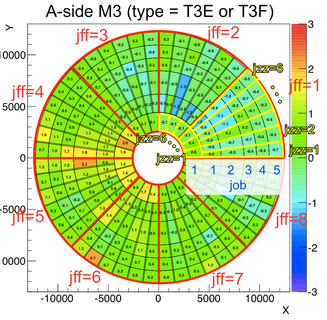
\includegraphics[clip, width=10cm]{fig/4/zure.png}
  \caption{Run-2での検出器のズレの測定図}
  \label{fig:ズレ}
\end{figure}


\subsection{検出器アライメント}
CW に対して検出器のズレを補正し最適化することで、トリガー効率を維持しつつ、トリガーレート削減を目指す。
Run-2で行われたシミュレーションを用いて作成した CW に対する TGC アライメントの補正方法について以下に述べる。


Run-2 では
2015 年 Run-2 の実データを用いた
この CW を cell 毎に判定する方法を CW optimization と呼ぶ。


・検出器アライメント
<山内さんの手法>
<木戸さんの手法の説明>


\section{本研究の目的}
Run-3における初段ミューオントリガーの性能を向上させるためには Run-2 と同様に CW の最適化を行う必要がある。しかし、\ref{section:最適化}節で述べたような Run-2 で行われていた最適化手法は、各CWごとに1マスずつ6段階の閾値を一段階ずつ確認する手法のため膨大な作業量が必要である。そのため、Run-3 で15段階に増設された閾値を持つ CW に対して Run-2 での最適化手法を行うことは現実的でない。
そこで、本研究では近年急速に発展している機械学習に着目し、新たな CW の最適化手法の開発を行う。















